\documentclass[border=7pt]{standalone}
\usepackage{tkz-euclide}
\usetkzobj{all} % on charge tous les objets

\begin{document}
  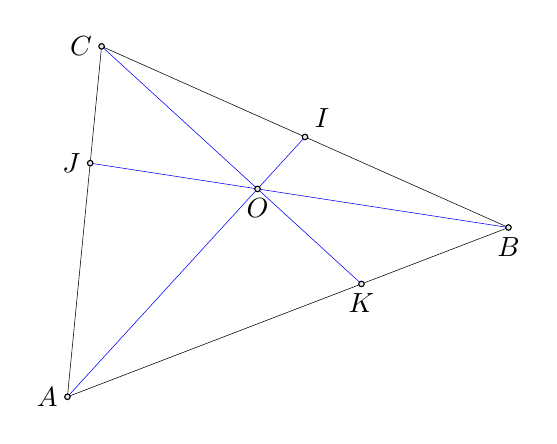
\begin{tikzpicture}[scale=2,rotate=21]
    % définition des points
    \tkzDefPoints{0/0/A, 3/0/B, 1/2/C, 2/1/I, 0.6666667/1.3333333/J, 2/0/K, 1.6/0.8/O}
    % tracer
    \tkzDrawSegments(A,B B,C C,A)
    \tkzDrawSegments[blue](A,I B,J C,K)
    % marquage des points
    \tkzDrawPoints(A,B,C,I,J,K,O)
    \tkzLabelPoints[below](B,K,O)
    \tkzLabelPoints[above right](I)
    \tkzLabelPoints[left](A,C,J)
  \end{tikzpicture}
\end{document}
\begin{tikzpicture}

\end{tikzpicture}
